\chapter{Python's threading model}
\label{cpt:pythons_thread_model}

\begin{figure}[t!]
	\makebox[\textwidth][c]{\includegraphics[width=\linewidth]{pythonthreading/diagrams/thread_io_release_diagram}}
	\caption{A schematic view of how threads release the GIL when performing IO in Python.}
	\label{fig:python_threads_release_gil}
\end{figure}

Python threads are normal operating system (OS) threads, either POSIX (pthread) or Windows threads \cite{beazley2010understanding, beazley2009inside}.
Also Python does not have a thread scheduler, threads are fully managed by the operating system that hosts them.
In the Python programming language there is a Global Interpreter Lock (GIL).
This GIL ensures that only one thread can run in the python interpreter at once, i.e. a thread needs to hold the GIL in order to execute.
This means there cannot be any parallel execution.
Once a thread is done executing or needs to wait it releases the GIL.
This gives way for cooperative multitasking as visualized in Figure \ref{fig:python_threads_release_gil}.
Other threads that are ready to execute can try to acquire the GIL, the thread that obtains the GIL is determined by the OS.

To make sure CPU heavy tasks do not hold the GIL indefinitely a simple check mechanism is built in that ``checks'' every thread once per 100 ticks.
Ticks are loosely mapped to interpreter instructions and do not define a time unit.
Listing \ref{lst:one_tick} contains two code samples that only take one tick each, but take require different amount of time to compute.

\lstinputlisting[caption={Two code samples that each take one tick yet require a different amount to compute.},label={lst:one_tick},language=Python]{pythonthreading/code/one_tick.py}

When a check is run the following four steps are executed:
\begin{enumerate}
	\item The thread that holds the GIL resets its tick counter.
	\item If the current thread it the main thread, it runs the signal handlers.
	\item The thread releases the GIL.
	\item The thread tries to reacquire the GIL.
\end{enumerate}

Note that a thread thus may or may not immediately reacquire the GIL after releasing it.
Since every thread has this check, CPU-bound threads will engage in cooperative multitasking.

\section{Multi threaded programming performance}
\label{sct:multi_theaded_programming_performance}

Since threads cannot run in parallel, this changes the performance one may expect from a multi-threaded program.
Dadiv Beazly presented his findings in his Python Concurrency Workshop (2009) \cite{beazley2009inside}.
By running a trivial CPU-bound function using two threads on a dual-core MacBook, processing time increased by 185\%.
Disabling one of his cpu cores yielded an increase of 154\% in run time.
To investigate this behaviour, Beazley inspected the underlying C code to inspect why he was observing these performance results.

Whenever a (Python) thread releases the GIL, it sends out a signal.
The OS then Propagates this signal to other threads which then can attempt to acquire the GIL.
The lag between thread switching and execution may be significant depending on the OS, according Beazley.
Most operating systems make use of a priority system for threads. 
The thread with the highest priority will be scheduled by the OS.
Often, CPU-bound threads have a low priority and I/O-bound threads a high priority.
If a signal is send to a low priority thread and all CPUs are currently busy processing other, high priority thread, it won't be run until one of the CPUs becomes available.

As it turns out, the GIL signalling is the source of the performance loss.
Whenever the ``check'' (see the previous Section) in run, the following happens:

\begin{itemize}
	\item First the Python interpreter locks a mutex.
	\item Next, it signals on a condition variable/semaphore where another thread is \emph{always} awaiting execution.
	\item Because of this waiting thread, additional pthread processing and system calls are generated to deliver the signal.
\end{itemize}

Beazley provided rough measurements on the number of system calls generated, summarized in Table~\ref{tbl:system_calls_thread_switching}.
From these numbers Beazley concludes that the overhead generated is significant and the main reason for the performance loss.
He then dived deeper into these numbers to find a cause.

By recording a real-time trace of all GIL related operations i.e. acquisition, release, etc., Beazley was able to reconstruct what happens.
When running multiple CPU-bound threads on multiple cores, all of them will be scheduled \emph{simultaneously}.
The threads proceed to battle over GIL acquisition. 
Whenever a thread releases the GIL because of the 100 tick ``check'', it immediately tries to reacquire it.
Another thread will also try to acquire the GIL upon this signal, but as this signal arrives with a delay it will most likely fail.
This processes is visualized by Figure~\ref{fig:gil_battle_threads} (David Beazley, 2009).
Beazley argues that here two competing goals are clashing.
On the one hand Python wants to only run one thread at a time and on the other hand the OS wants to schedule as many processes/threads to take advantage of its cores.
This clash raises a lot of overhead, which results in a severe performance penalty.

Even when running the threads on one core results in these battles.
I/O-bound threads which are high priority may fail to acquire the GIL when a CPU-bound thread is busy.
This degrades the response time of the I/O thread.

 \begin{figure}[t!]
 	\makebox[\textwidth][c]{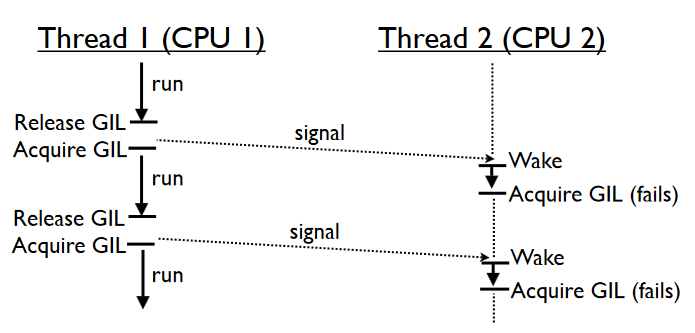
\includegraphics[width=\linewidth]{pythonthreading/images/gil_battle_threads}}
 	\caption{A schematic view of two threads battling for GIL acquisition (source: David Beazley, 2009).}
 	\label{fig:gil_battle_threads}
 \end{figure}

\begin{table}[]
	\centering
	\begin{tabular}{|l|l|l|l|}
		\hline
	\textbf{Threads}	& \textbf{Cores} & \textbf{Unix system calls} & \textbf{Mach system calls} \\ \hline
	1	& 1 & 736 & 117 \\ \hline
	2	& 1 & 1149 & 3.3M \\ \hline
	2	& 2 & 1149 & 9.5M \\ \hline
	\end{tabular}
	\caption{A summary of the rough measurements from David Beazley \cite{beazley2009inside}.}
	\label{tbl:system_calls_thread_switching}
\end{table}



\section{Asynchronous programming}

\todo{In the problem description is explain why asynchrony helps resolving IO bottlenecks, what should be put here?}